%%%%%%%%%%%%%%%%%%%%%%%%%%%%%%%%%%%%%%%%%%%%%%%%
% 1. Document class 
\documentclass[a4paper,12pt]{article} % This defines the style of your paper
%%%%%%%%%%%%%%%%%%%%%%%%%%%%%%%%%%%%%%%%%%%%%%%%
% 2. Packages
\usepackage[top = 2.5cm, bottom = 2cm, left = 2cm, right = 2.5cm]{geometry} 
\usepackage[T1]{fontenc}
\usepackage[utf8]{inputenc}
\usepackage{multirow} % Multirow is for tables with multiple rows within one cell.
\usepackage{booktabs} % For even nicer tables.
\usepackage{graphicx} 
\usepackage{setspace}
\setlength{\parindent}{0in}
\usepackage{float}
\usepackage{fancyhdr}
\usepackage{titlesec}
\usepackage{url}
\usepackage{amsmath,amssymb,amsthm,bm}
\usepackage{subcaption}
\usepackage{clrscode3e}

\newcommand{\problemAnswer}[1]{ % Defines the problem answer command with the content as the only argument
\noindent\framebox[\columnwidth][c]{\begin{minipage}{0.98\columnwidth}#1\end{minipage}} % Makes the box around the problem answer and puts the content inside
}

\titleformat*{\section}{\large\bfseries}
\titleformat*{\subsection}{\bfseries}
%%%%%%%%%%%%%%%%%%%%%%%%%%%%%%%%%%%%%%%%%%%%%%%%
% 3. Header (and Footer)
\pagestyle{fancy} % With this command we can customize the header style.
\fancyhf{} % This makes sure we do not have other information in our header or footer.
\lhead{\footnotesize  CS 5200}% \lhead puts text in the top left corner. \footnotesize sets our font to a smaller size.
%\rhead works just like \lhead (you can also use \chead)
\rhead{\footnotesize Project Proposal} %<---- Fill in your lastnames.
% Similar commands work for the footer (\lfoot, \cfoot and \rfoot).
% We want to put our page number in the center.
\cfoot{\footnotesize \thepage} 

\begin{document}
\thispagestyle{empty} % This command disables the header on the first page. 

\begin{tabular}{p{15.5cm}} % This is a simple tabular environment to align your text nicely 
{\large \bf CS 5200 Database Management Systems} \\
Northeastern University, Spring 2019  \\
\hline % \hline produces horizontal lines.
\end{tabular} % Our tabular environment ends here.

\vspace*{0.3cm} % Now we want to add some vertical space in between the line and our title.

\begin{center} % Everything within the center environment is centered.
    {\Large \bf Project Proposal} % <---- Don't forget to put in the right number
    \vspace{2mm}
    
        % YOUR NAMES GO HERE
    {Name: Zihan Liu UID: 001880907}\\
    {Name: Yuan Gao UID: 001202419}\\
    {Github: https://github.com/Cappuccinuo/NBA\_DB}
\end{center} 
%
\vspace{0.2cm}
\section{Top Level Description}
The project is a NBA data statistics website for one specific season. 
The data domains contain games, teams and players related data. The user can do the following things in our website:\\
1.Display the statistical data of players and teams in one game, as well as player and team information.\\
2.Insert new players and new teams.\\
3.Update the information of games, teams and players.\\
4.Delete one specific game, team or player.\\
5.Query the data using multiple filter, e.g. Search for the team which can average score more than 100 and have less
than 10 average turnovers each game.
\section{SQL vs NO SQL storage}
We choose relational database(SQL) as our main storage. The reason is that our data is structural and 
well-formed, and many RDBMS have a good balance between durability and performance when doing ACID. 
For RDBMS, we choose MySQL which is most used by us.

\section{Hardware and Software}
DBMS: MySQL\\[5pt]
Visual database design tool: MySQL Workbench\\[5pt]
Software: Sublime \& Intellij\\[5pt]
Front-end web framework: Angular\\[5pt]
Back-end development: Java (JDBC)\\[5pt]
All of above are cross-platform and open-source.\\[5pt]
Hardware: No restrictions
\section{Why does this project or this data domain interest you?}
a. NBA is one of the most popular sports around the world. NBA fans need an easy way to obtain 
the up-to-date information of the league and customize their query. 
At the same time, the manager of the team require an easy way to query and maintain the data. \\[5pt]
b. NBA is the best sport league in the world, it has rich data for us to explore.\\[5pt]
c. Our favoriate sport is basketball, we want to conduct a project related to this field.
\section{UML diagram}
\begin{center}
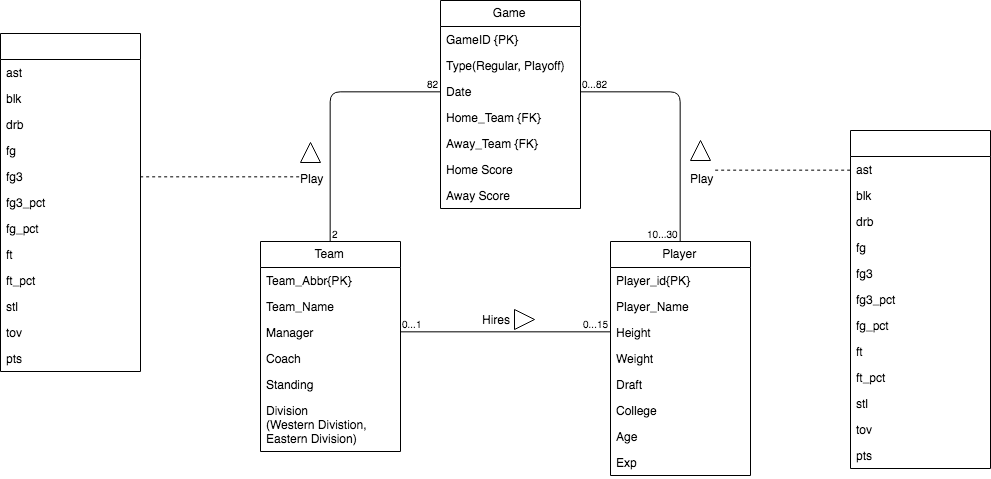
\includegraphics[width=1\textwidth]{NBA}
\end{center}
\section{Step by step user interaction}
\begin{center}
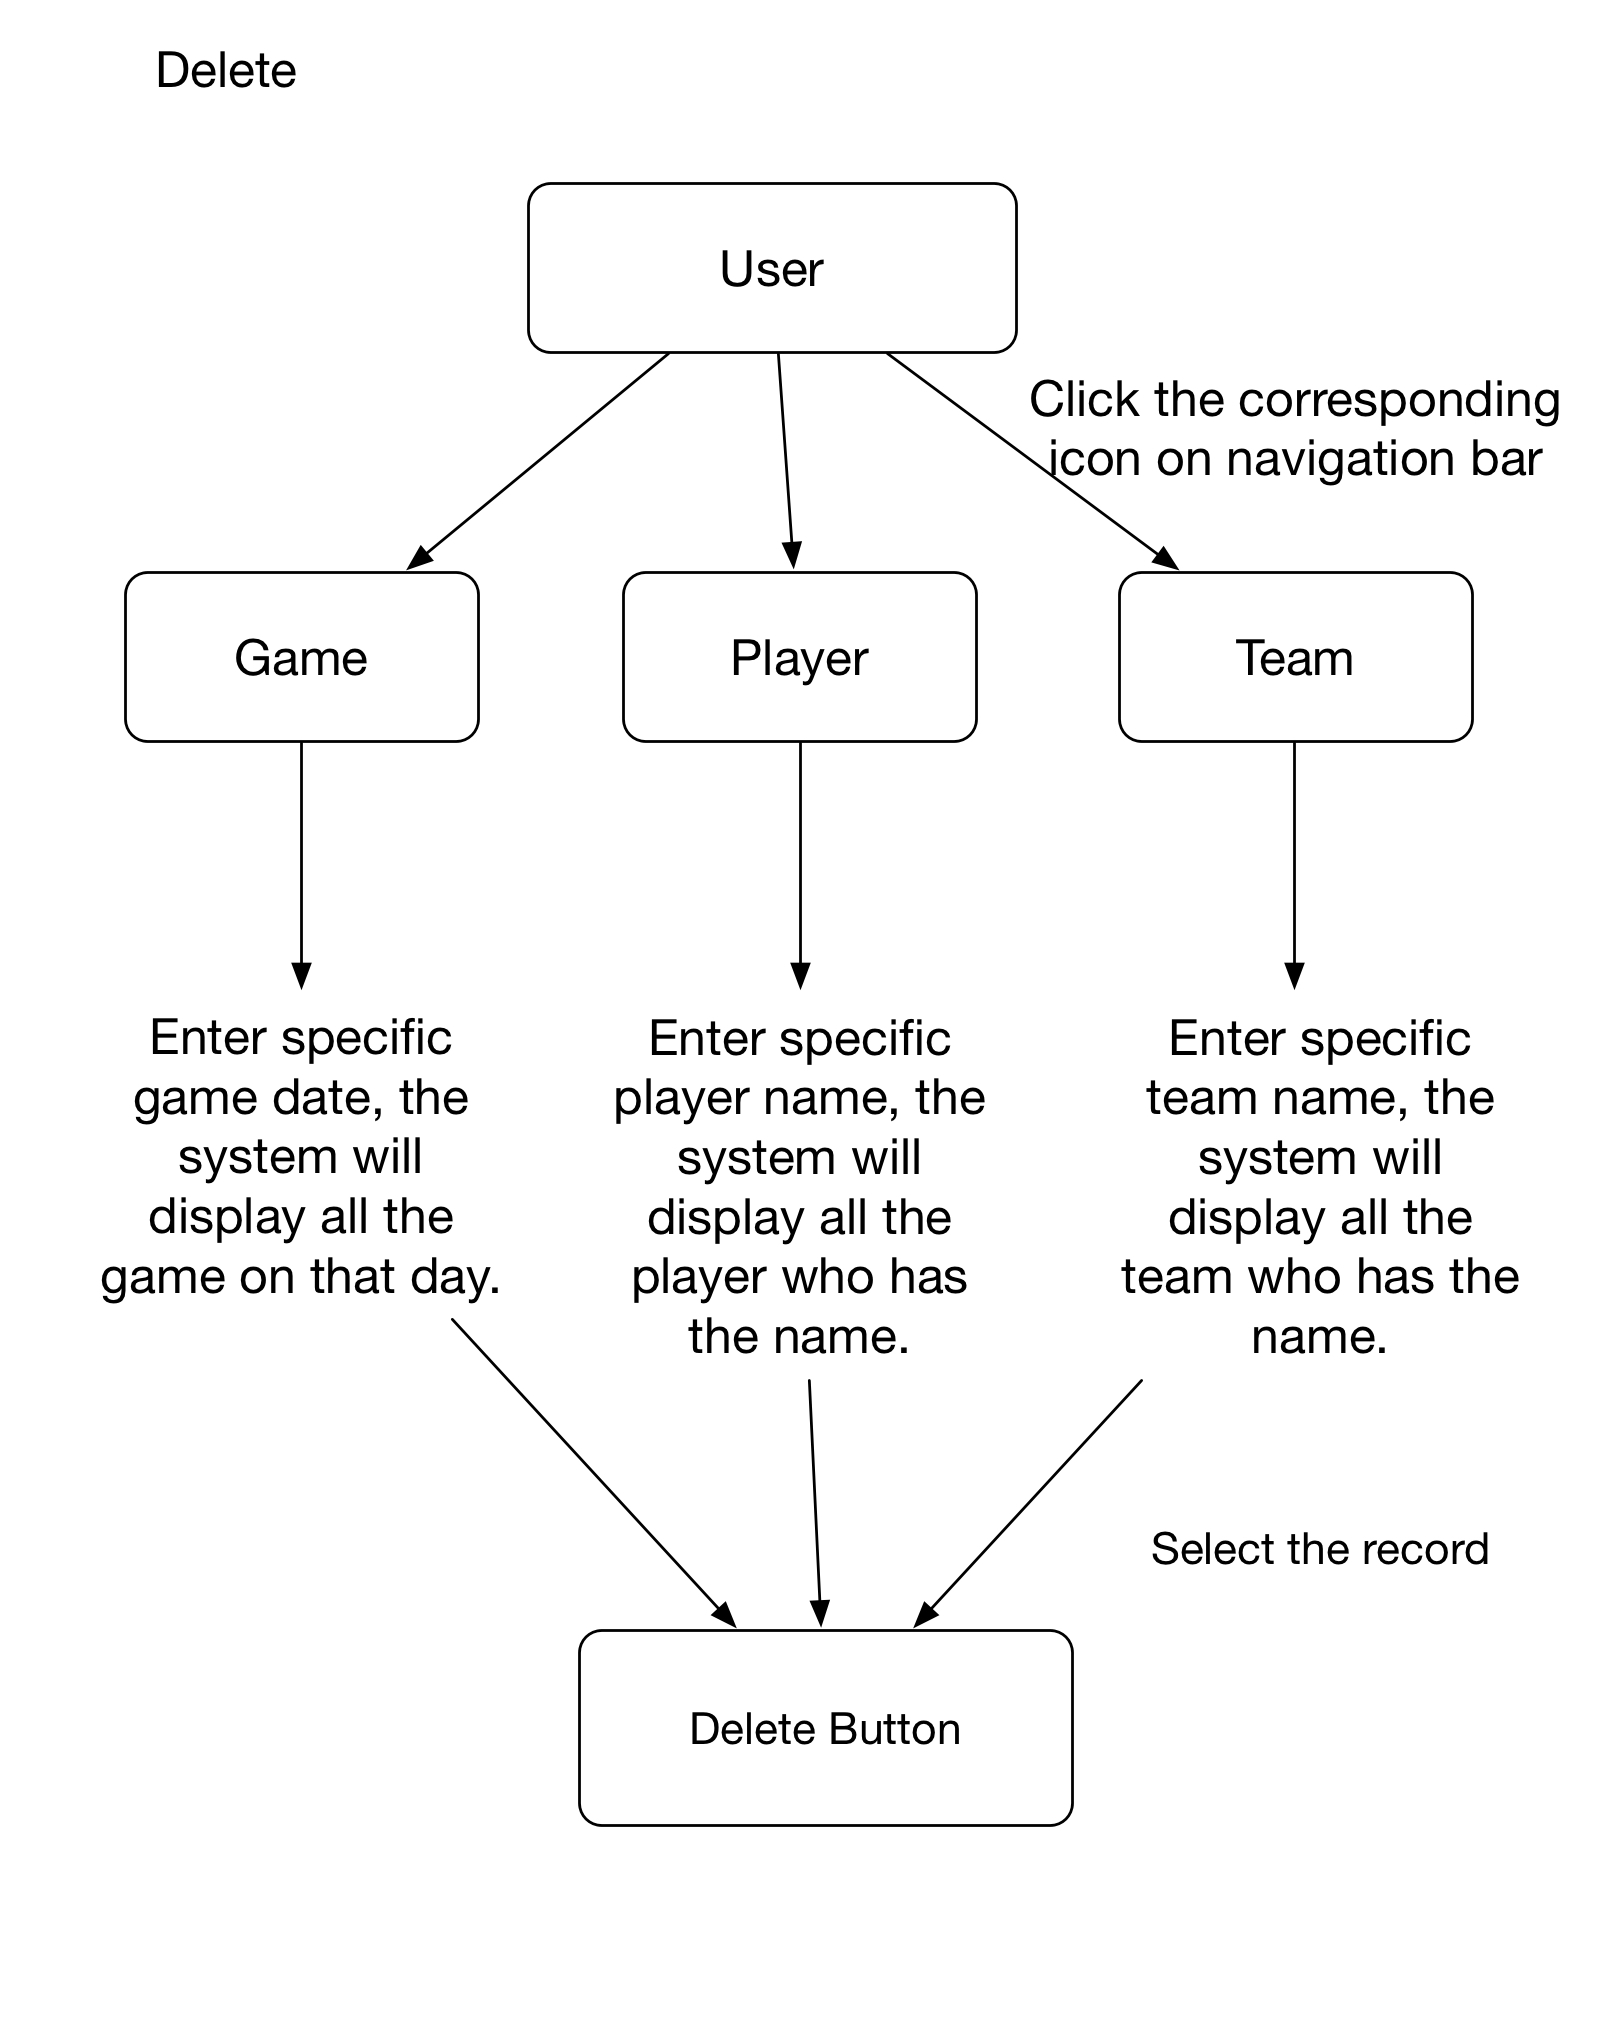
\includegraphics[width=1\textwidth]{DeleteChart}
\end{center}
\begin{center}
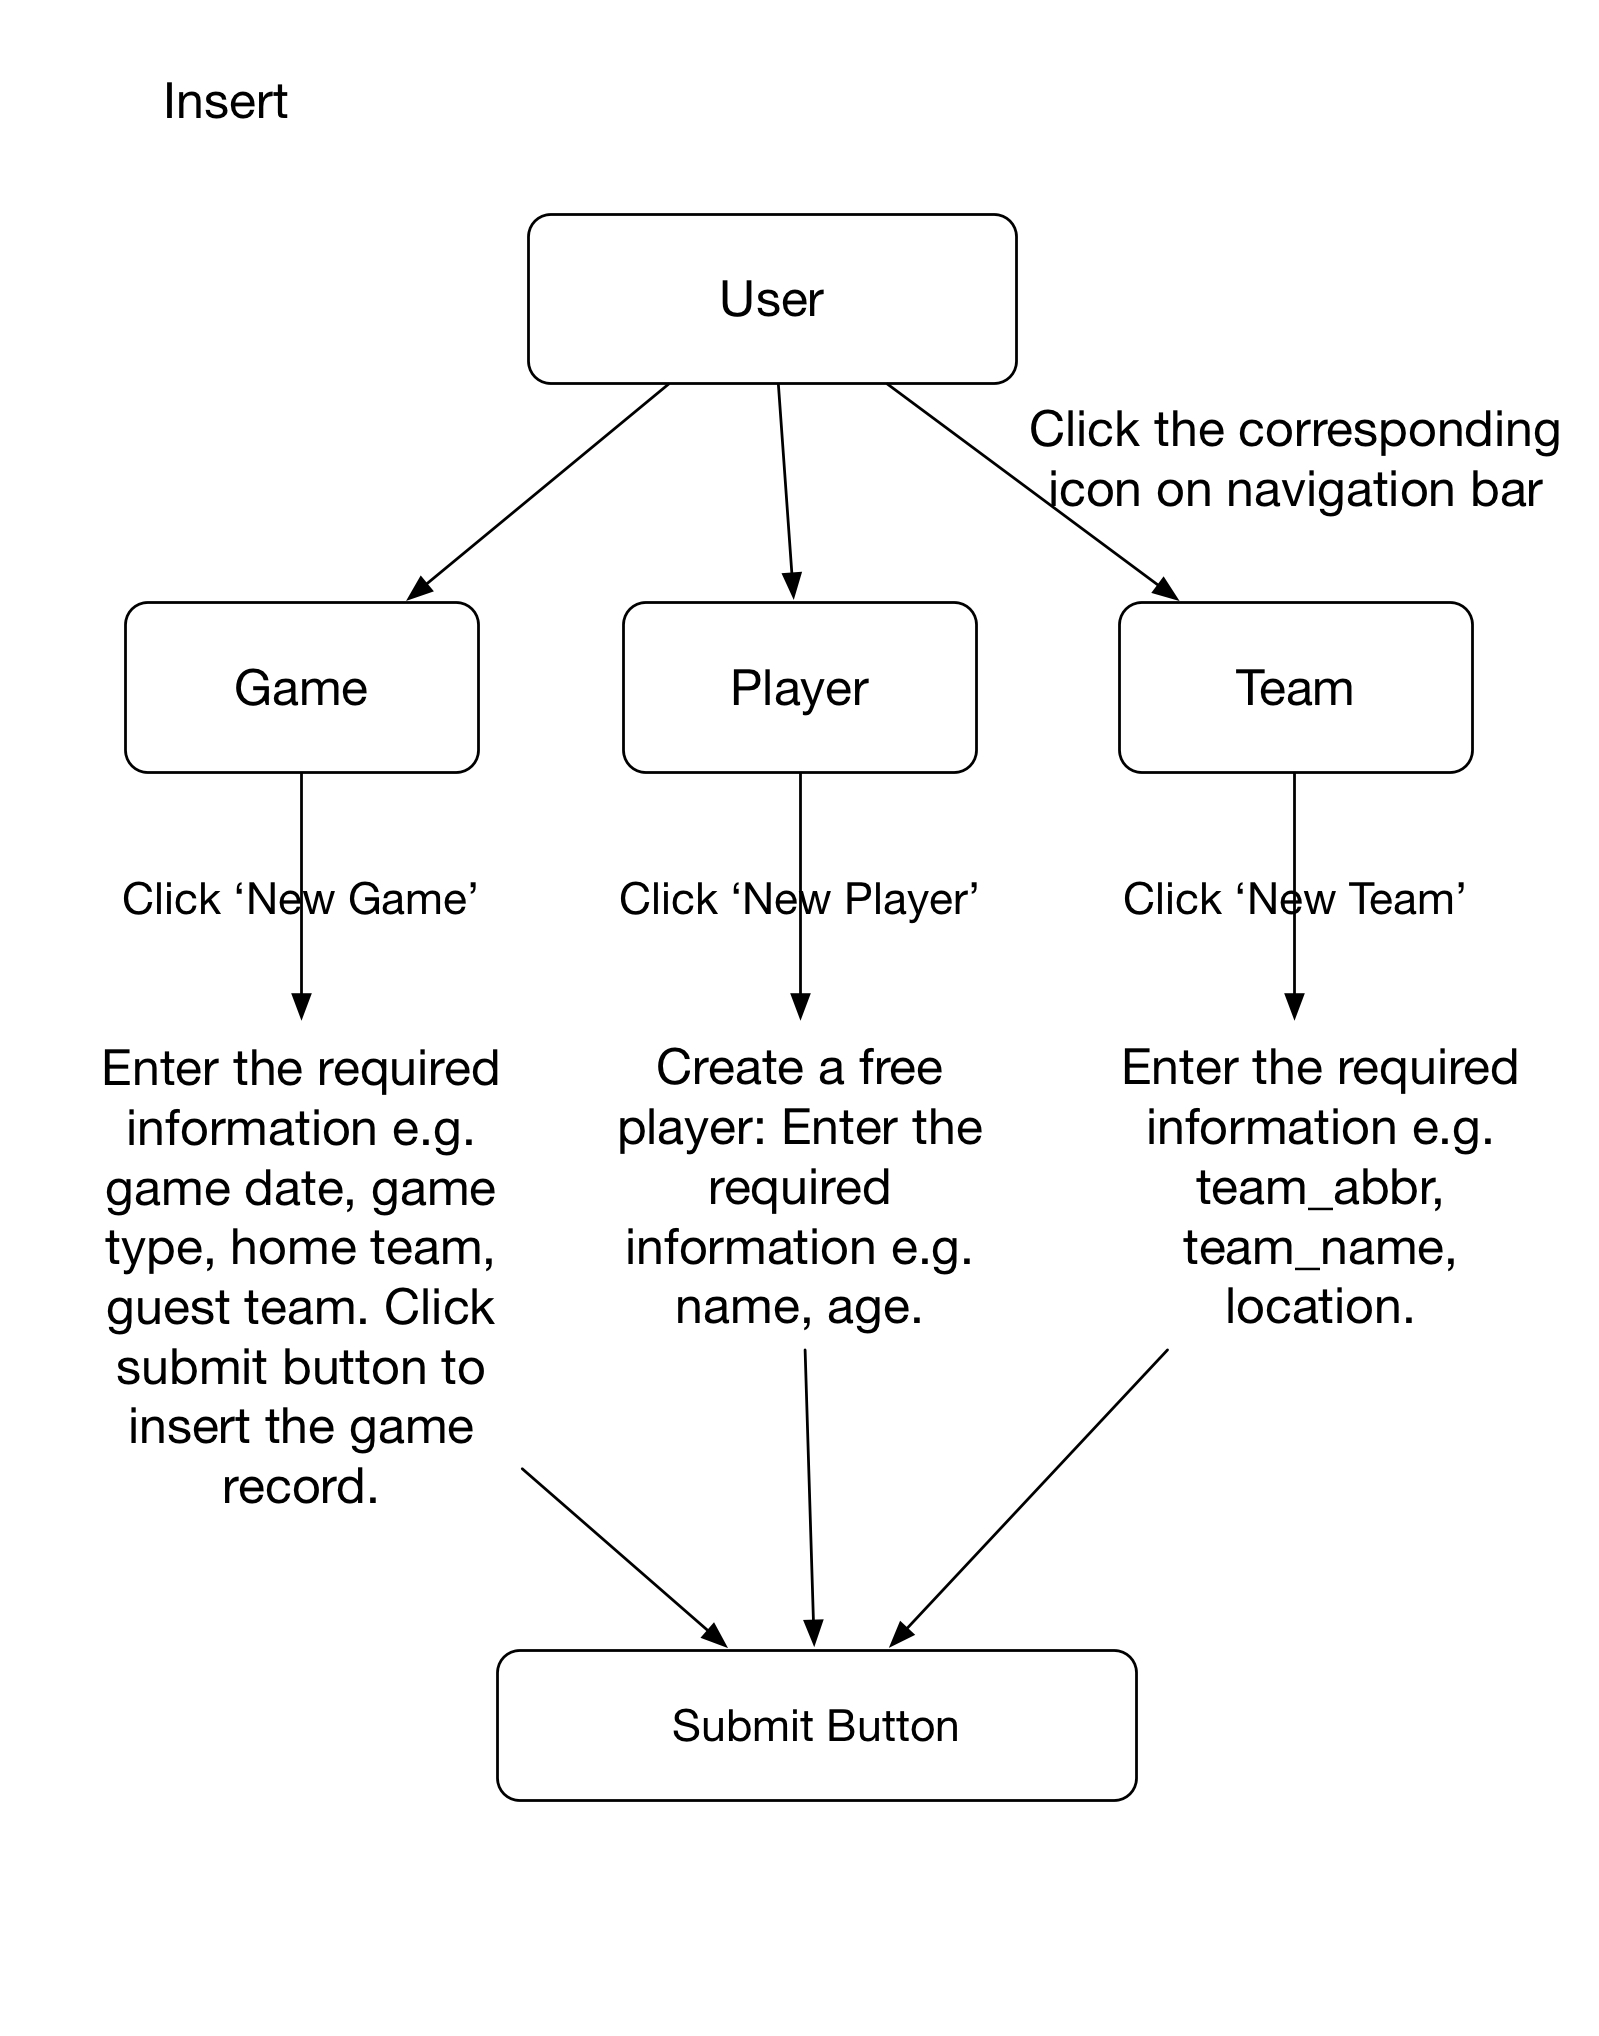
\includegraphics[width=1\textwidth]{InsertChart}
\end{center}
\begin{center}
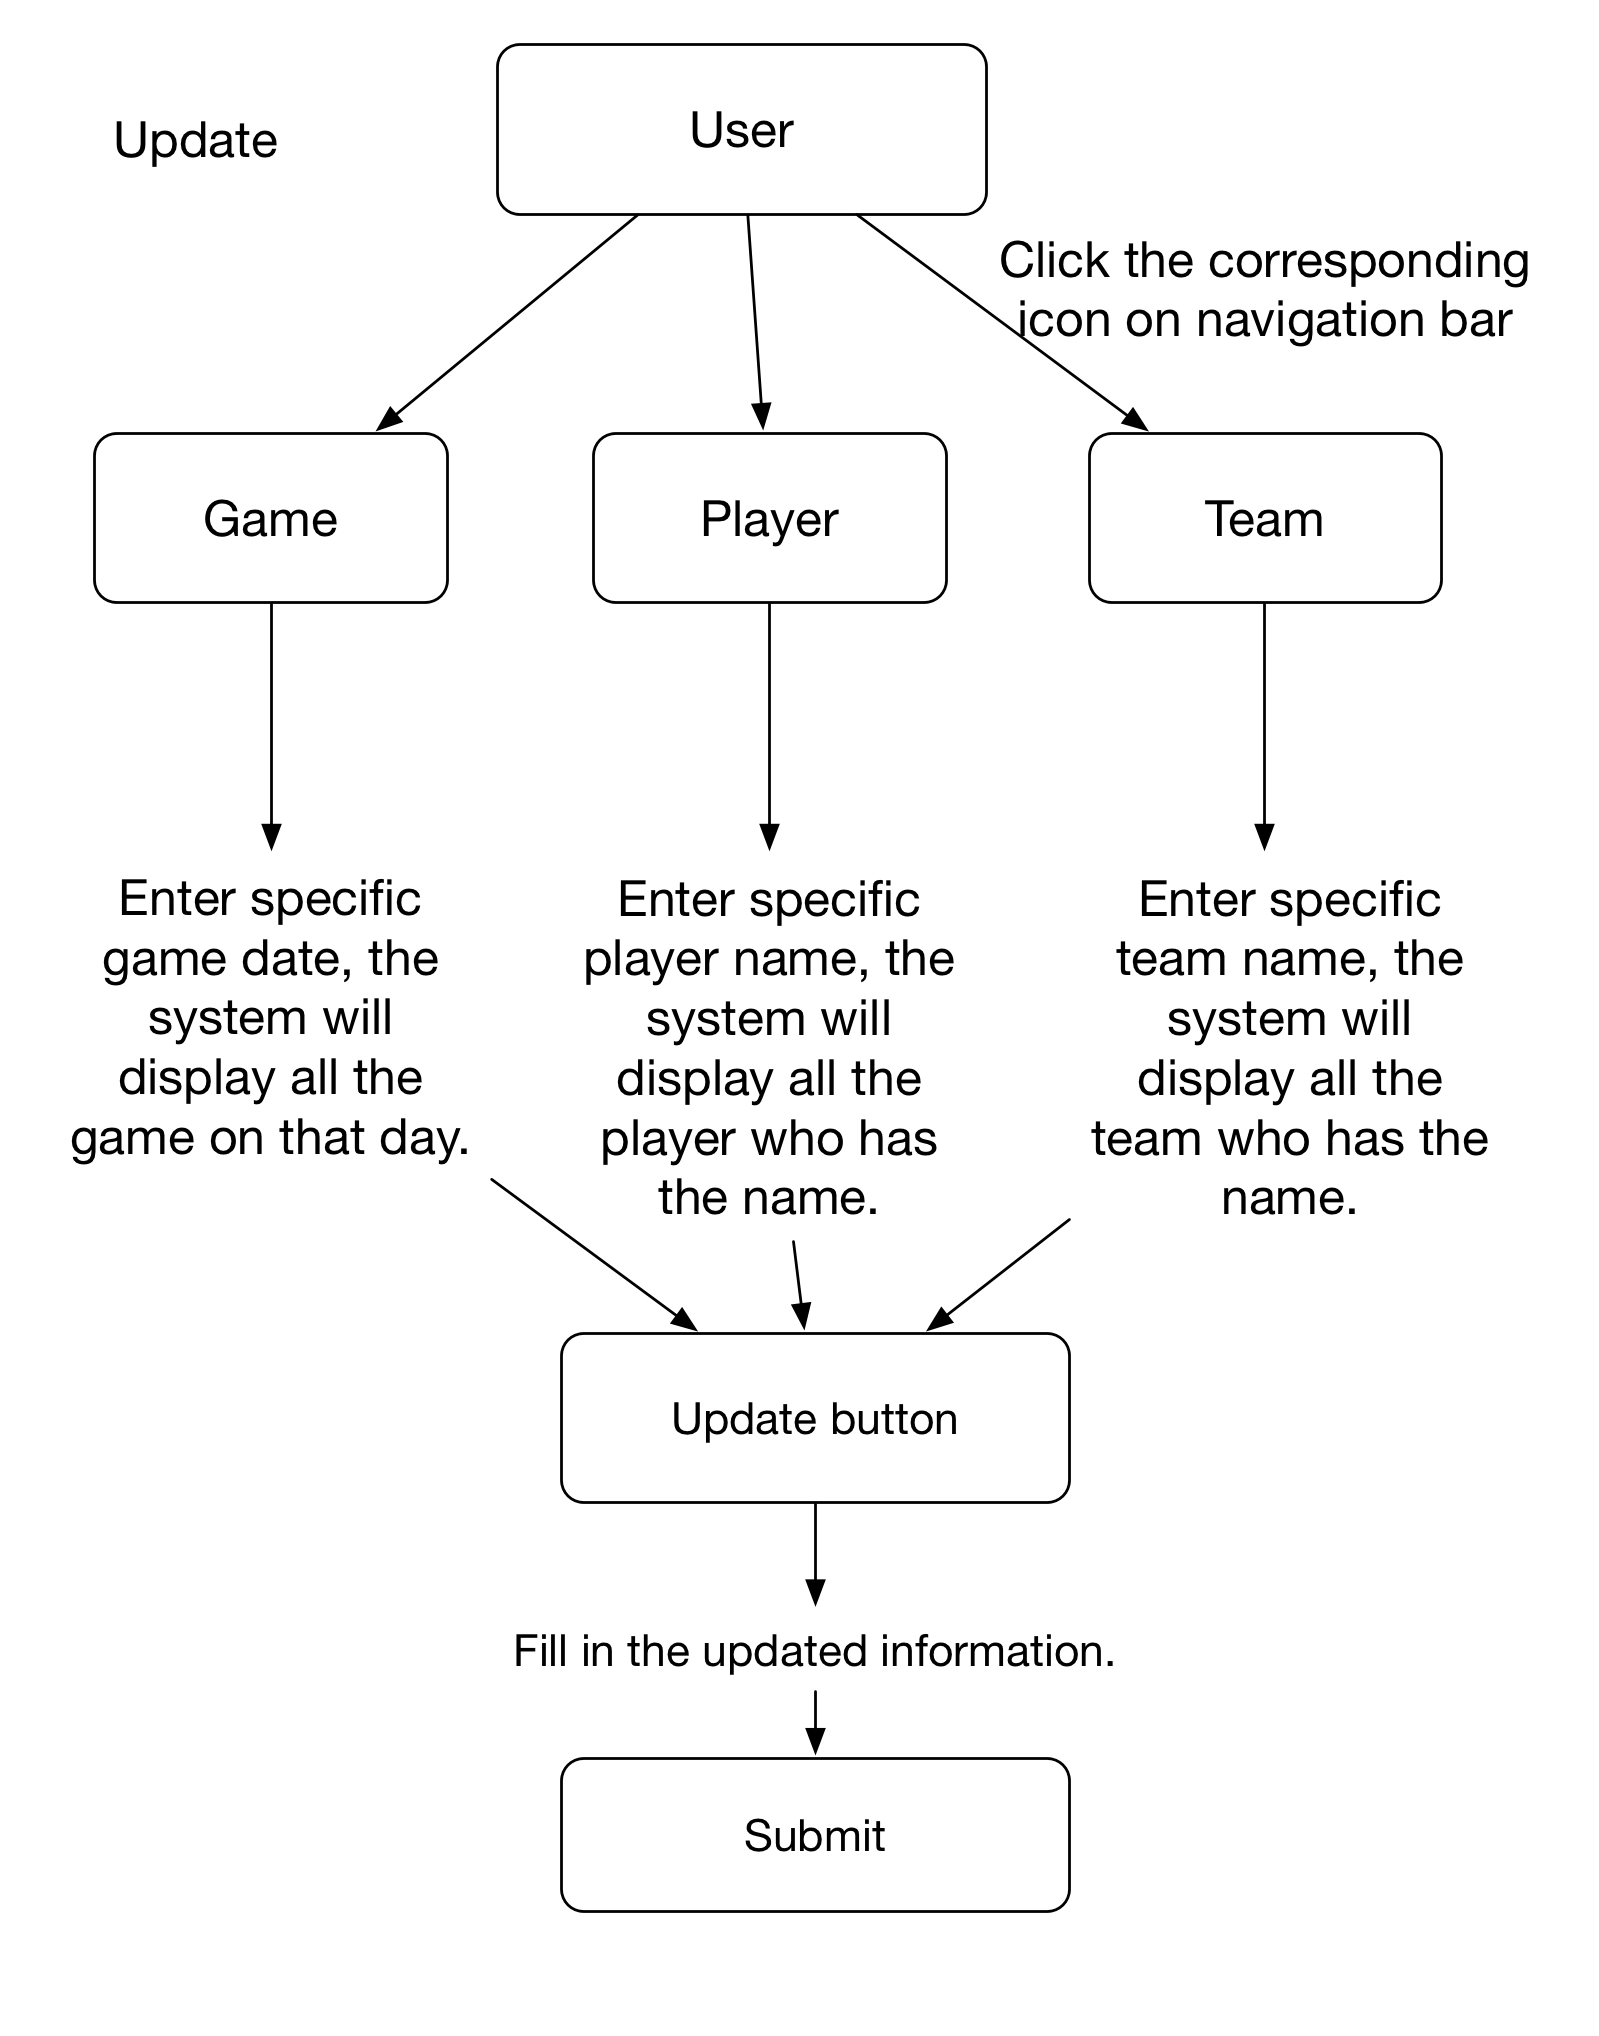
\includegraphics[width=1\textwidth]{UpdateChart}
\end{center}
\begin{center}
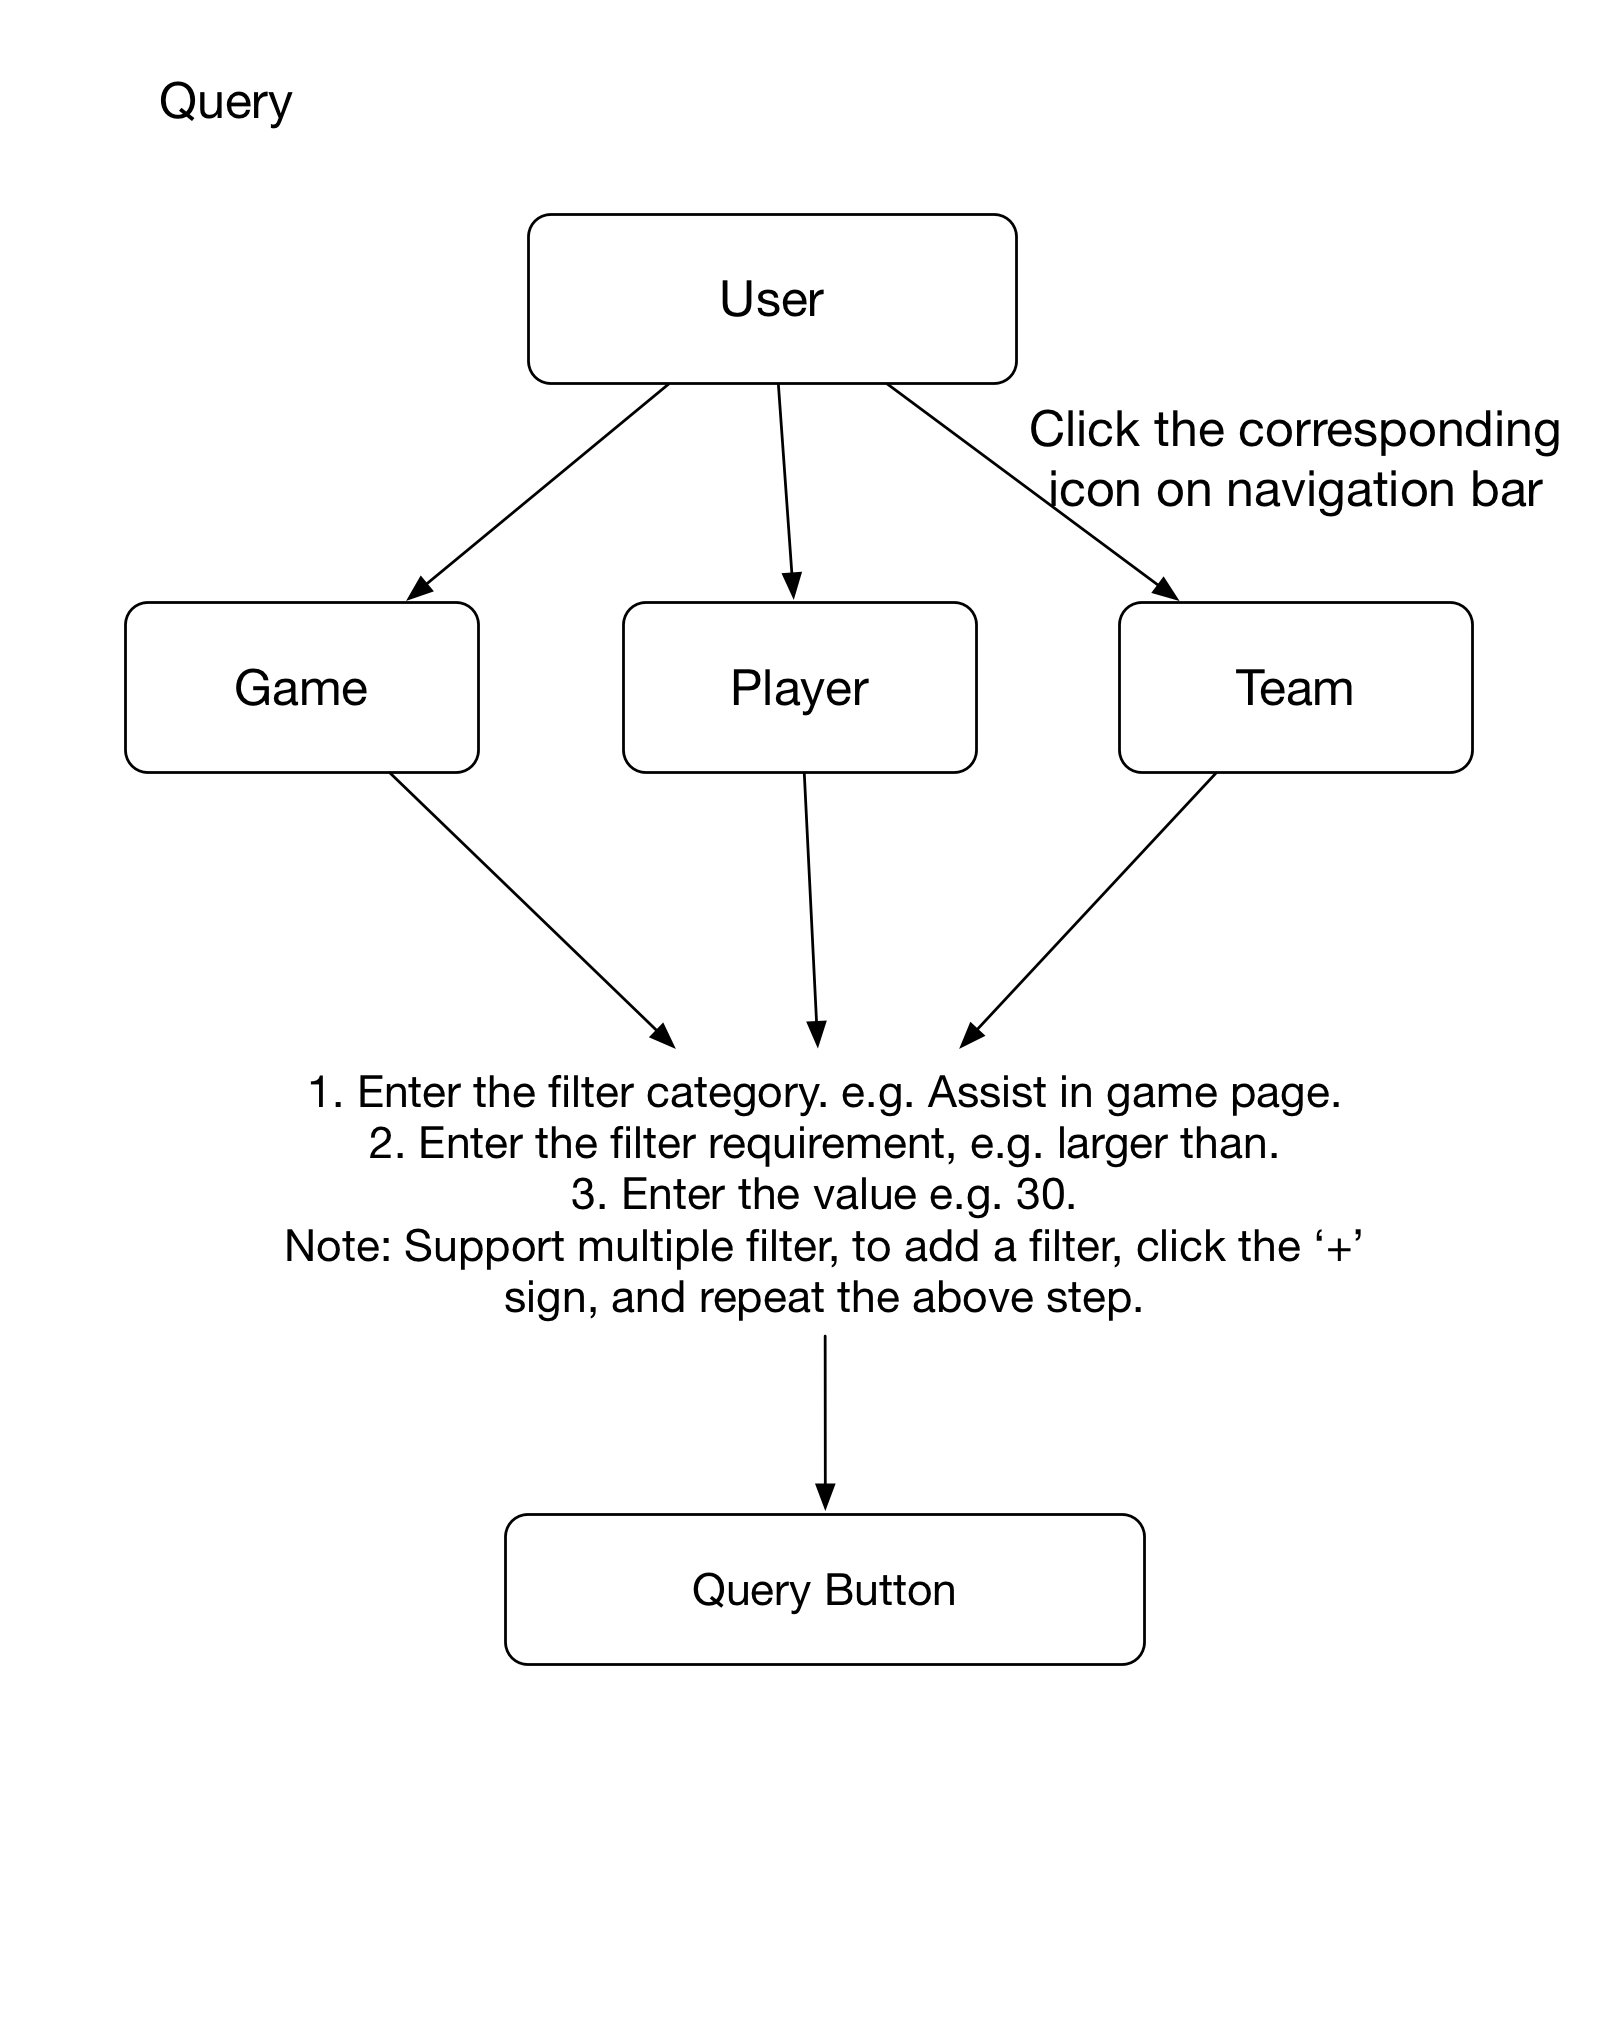
\includegraphics[width=1\textwidth]{QueryChart}
\end{center}
\end{document}